\section{Query expansion}
\subsection{Motivation}

If the user query does not contain a relevant term, the corresponding
documents will not show up in the result.
Example: query ``car'' will not return ``automobile''.
Question: How to add such documents (increase recall)?

\texttt{Idea}: System adds query terms to user query!

\subsection{Two methods}
\begin{itemize}
\item Local approach \\
  Use information from current query results: \textbf{user relevance
    feedback}
\item Global approach: \\
  Use information from a \textbf{document collection}: \texttt{query
    expansion}
\end{itemize}

\subsection{User relevance feedback}

Reformulate a query by taking into account feedback of the user on the
relevance of already retrieved documents.
Advantages:
\begin{itemize}
\item The user is not involved in query formulation, just points out
  relevant results.
\item The search task can be split up in smalller steps
\item The search task becomes a process converging to the desired
  result.
\end{itemize}

Relevant documents $ C_r $, some retrieval result $ R $.
$ D_r \subset C_r \cap R  $, and $ D_n \subset R \setminus C_r $

\subsection{Collection centroid}

$ \omega(D) = \frac{1}{\| D \|} \sum_{d \in D} \vec{d} $

\textit{Rocchio algorithm}: find query that optimally separates
relevant from non-relevant documents

$ \vec{q_opt} = argmax_{\vec{q}}[sim(\vec{q}, \omega(D_r)) -
sim(\vec{q}, \omega(D_n))] $

The centroid of all document vectors of a document set can be
considered as most characteristic representation of the document
set. Then one could attempt to construct a query $ q_{opt} $  that
optimally separates relevant documents from non-relevant ones. In
order to achieve this, the query to be constructed has to have maximal
similarity with the set of relevant documents, respectively its
centroid, and maximal dissimilarity with the set of non-relevant
documents, respectively its centroid. This can be achieved by a query
that maximizes the difference among these two similarity values.

\subsection{Identifying relevant documents}

We then have $ \vec{q_{opt}} = \omega(D_r) + [\omega(D_r) -
\omega(D_n)] $

\texttt{Issues}:
\begin{itemize}
\item User relevance is not complete
\item User do not always identify non-relevant documents
\item Original query should continue to be considered
\end{itemize}

\subsection{SMART}

Approximation scheme for the theoritcally optimal query vector.
If users identify some relevant documents $ D_r  $ from the result set
R of a retrieval query q.
\begin{itemize}
\item Assume all elements in $ R \setminus D_r $ are not relevant, i.e.\
  $ D_n = R \setminus D_r $
\item Modify the query to approximate theoretically optimal query
  $ \vec{q_approx} = \alpha \vec{q} + \frac{\beta}{\| D_r \|} \sum_{\vec{d_j} \in D_r} \vec{d_j}
  - \frac{\gamma}{\| R \setminus D_r} \sum_{\vec{d_j} \notin D_R}
  \vec{d_j}$
\item $ \alpha, \beta, \gamma $ are tuning parameters, $ \alpha, \beta,
  \gamma \geq 0 $
\end{itemize}

This method assumes that users have identified some relevant documents
and considers all other documents as non-relevant. The modification of
the query is controlled by the 3 parameters.

Moderate the impact of this wrong assumption:
\begin{itemize}
\item Original query vector is maintained, in order not to drift away
  too far from the original user query
\item The weight given for the modification using the centroid of
  non-relevant documents is kept lower than that of the centroid of
  relevant documents.
\end{itemize}

Underlying assumptions of SMART:
\begin{itemize}
\item Users has sufficient relevant terms in initial query
\item Results contain additional temrs together with original terms
\item Users are willing to provide feedback!!!
\end{itemize}

\subsection{Pseudo-relevance feedback}

If users do not give feedback, automate the process:
\begin{itemize}
\item Choose the top-k documents as relevant ones
\item Apply SMART
\end{itemize}

Works often weel, but can fail horribly in some case: query drift.

\subsection{Global Query Expansion}

Query is expanded using a global, query-independent resource:
\begin{itemize}
\item Manually edited thesaurus
\item Automatically extracted thesaurus, using term co-occurence
\item Query logs
\end{itemize}

\subsubsection{Manually created thesaurus}
Expensive to maintain and create. Used mainly in science and
engineering (Pubmed)

\subsubsection{Automatic thesaurus generation}
Generate a thesaurus automically by analyzing word distribution of
documents. Idea: \textit{similarity between two words}

Two words are similar if they \textbf{co-occur} with similar
words. ``switerzland'' $ \approx $ ``austria'' because both occur with
such as ``national'', ``election'', ``soccer'', etc., so they must be
similar.

Two words are similar if the occur in a given grammatical relation
with the same words. ``live in \%'', ``travel to \%''\ldots are all
phrases in which both ``switzerland'' and ``austria'' can occur.

\subsubsection{Expansion using query logs}
Main source of query expansion at search engines.
Exploit correlation in user sessions

Example 1: \textit{users extend query}
\begin{itemize}
\item After searching Obama, users search Obama president
\item Therefore, president might be a good expansion
\end{itemize}

Example 2: \textit{users refer to same result}
\begin{itemize}
\item User A accesses URL epfl.ch after search Aebischer
\item User B accesses URL epfl.ch after search Vetterli
\item Vetterli might be an expansion for the query Aebischer and
  vice-versa.
\end{itemize}

\subsection{Indexing for IR}

\subsubsection{Term search}
Problem: text retrieval algorithms need to find words in document
efficiently:
\begin{itemize}
\item Boolean retrieval, probabilistic and vector space retrieval
\item Given index term $ k_i $, find document $ d_j $
\end{itemize}

\subsubsection{Inverted files}

An inverted file is a word-oriented mechanism for indexing a text
collection in order to speed up the term search task
\begin{itemize}
\item Addressing of documents and words position within documents
\item Most frequently used indexing technique for large text DBs
\item Appropriate when text collection is large and semi-static
\end{itemize}

Frequent updates are not supported with inverted files. This is different from
typical database indexing techniques (e.g.\ B+-trees).

Inverted list $ l_k $ for a term k

$ l_k = \{ f_k : d_{i_1}, \ldots, d_{i_fk} \} $
\begin{itemize}
\item $ f_k $ number of documents in which k occurs
\item $ d_{i1}, \ldots, d_{ifk} $ list of document identifiers
  contains k
\end{itemize}

Inverted files: lexicographically ordered sequence of inverted lists:
$ IF = \{ i, k_i, l_{k_i} \}, \, i = 1, \ldots, m $

Storing the frequency is useful for computing term frequency and
inverse document frequency.

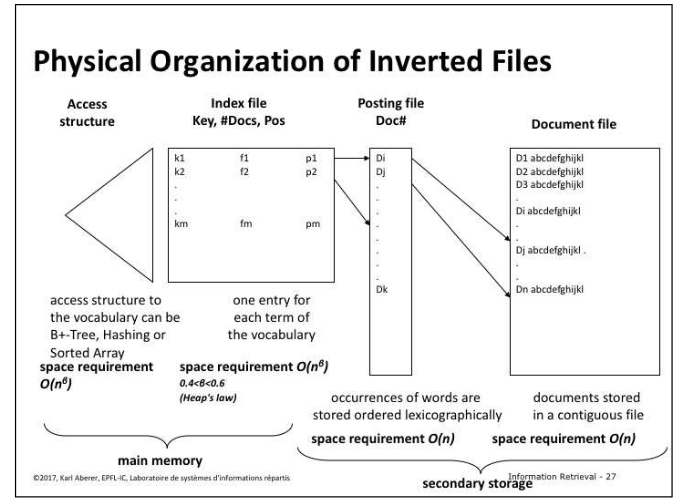
\includegraphics[height=150px,width=220px]{IF.png}

\subsubsection{Searching the inverted file}

\begin{itemize}
\item Step 1: Vocabulary search
  \begin{itemize}
  \item the words present in the query are searched in the index file.
  \end{itemize}
\item Step 2: Retrieval of occurences
  \begin{itemize}
  \item the lists of occurences of all words found are retrieved from
    the posting file.
  \end{itemize}
\item Step 3: Manipulation of occurences
  \begin{itemize}
  \item the occurences are processed in the document file to process
    the query.
  \end{itemize}
\end{itemize}

\subsubsection{Construction of the inverted file}

\begin{itemize}
\item Step 1: search phrase
  \begin{itemize}
  \item The vocabulary is kept in a trie data structure storing for
    each word a list of its occurences
  \item Each word of the text is read sequentially and searched in the
    vocabulary
  \item If it is not found, it is added to the vocabulary with an
    empty list of occurences
  \item The word position is adde dto the end of its list of
    occurences
  \end{itemize}
\item Step 2: storage phase
  \begin{itemize}
  \item The list of occurences is written contiguously to the disk
    (posting file)
  \item The vocabulary is stored in lexicographical order (index file)
    in main memory together with a pointer for each word to its list
    in the posting file
  \end{itemize}
\end{itemize}

Using a trie in index construction:
\begin{itemize}
\item helps to quickly find words that have been seen before
\item helps to quickly decide whether a word has not been seen before
\item helps to maintain lexicographic order of words seen in the
  document
\end{itemize}

\subsubsection{Construction in practice}
When using a single node not all index information can be kept in main
memory $ \rightarrow $ index merging:
\begin{itemize}
\item When no more memory is available, a partial index $ l_i $ is
  written to disk
\item The main memory is erased before continuing with the rest of the
  text
\item Once the text is exhausted, a number of partial indices $ l_i $
  exist on disk
\item The partial indices are merged to obtain the final index
\end{itemize}

\subsubsection{Web-scale index construction: Map-Reduce}

Pioneered by Google: 20 PB of data per day.
\begin{itemize}
\item Scan 100TB on 1 node @ 50MB/s = 23 days
\item Scan on 100-node cluster = 33 min
\end{itemize}

Cost-efficiency:
\begin{itemize}
\item Commodity nodes, network (cheap, unreliable)
\item Automatic fault-tolerance (fewer admins)
\item Easy to use (fewer programmers)
\end{itemize}

\textbf{Map-Reduce programming model}

Data type: key-value pairs $ (k, v) $ \\
Map function: $ [(k_{in}, v_{in})] \rightarrow [(k_{inter},
v_{inter})] $
Reduce function: $ (k_{inter}, [v_{inter}]) \rightarrow [(k_{out},
v_{out})] $

\textbf{Map-Reduce processing}

The document collection is partitionned and assigned to different
mapper nodes. The mapper nodes extract word statistics for their
partition of the document collection. For each word a reducer node is
responsible. Based on the key, i.e.\, a word, the mapper nodes sent
their local results for the word to the responsible reducer node. The
reducer node aggregates the statistics that they receive from all
mapper nodes. Once the reducer nodes have finalized generating the
partial indices for their key space, the results are written to the
file system by an output writer node.

\subsection{Addressing granularity}

Documents can be addressed at different granularity
\begin{itemize}
\item coarser: text blocks spanning multiple documents
\item finer: paragraph, sentence, word level
\end{itemize}

General rule
\begin{itemize}
\item the finer the granularity the less post-processing but the
  larger the index
\end{itemize}

The posting file has the most space requirements. Three addressing
scheme exist:
\begin{itemize}
\item Exact word position
\item Occurence within a document
\item Occurence with an arbitrary sized block = equally sized
  partitions of the document collection
\end{itemize}

The larger the granularity the fewer entries occur in the posting
file. In turn, additional post-processing required in order to
determine exact positions of index terms.

\subsection{Index compression}

Documents are ordered and each document identifier $ d_{ij} $ is
replaced by the difference to the preceding document identifier.
\begin{itemize}
\item Document identifiers are encoded using fewer bits for smaller,
  common numbers \\
  $ l_k = (f_k : d_{i_1}, \ldots, d_{i_{fk}}) \rightarrow
  l_k = (f_k : d_{i_1}, d_{i_2} - d_{i_1}, \ldots, d_{i_{fk}} -
  d_{i_{fk} - 1}) $
  \item Use of varying length compression further reduces space
    requirements
\end{itemize}

%%% Local Variables:
%%% mode: latex
%%% TeX-master: "master"
%%% End:
